\documentclass[../../thesis.tex]{subfiles}

\begin{document}
\begin{figure}[tb]
    \centering
    \pgfdeclarelayer{bg}    % declare background layer
    \pgfsetlayers{bg,main}  % set the order of the layers (main is the standard layer)
    \tikzsetnextfilename{membrane_distribution}
    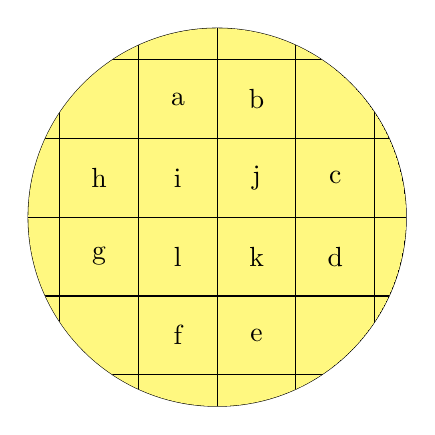
\begin{tikzpicture}
            \clip[draw] (-1,-7) circle (2.4);
            \fill[yellow!50] (-1,-7) circle (2.4);
            \node at (-1.5,-5.5) {a};
            \node at (-0.5,-5.5) {b};
            \node at (0.5,-6.5) {c};
            \node at (0.5,-7.5) {d};
            \node at (-0.5,-8.5) {e};
            \node at (-1.5,-8.5) {f};
            \node at (-2.5,-7.5) {g};
            \node at (-2.5,-6.5) {h};
            \node at (-1.5,-6.5) {i};
            \node at (-0.5,-6.5) {j};
            \node at (-1.5,-7.5) {l};
            \node at (-0.5,-7.5) {k};
            \draw[step=1] (-4,-10) grid (2,-4);
    \end{tikzpicture}
    \caption{Convention used to assign membrane depending on their position on the wafer.}
    \label{fig:membrane-distribution}
\end{figure}
\end{document}
